\documentclass[12pt]{report}
\usepackage[utf8]{inputenc}
\usepackage[russian]{babel}
\usepackage{setspace} % для междустрочного интервала
\onehalfspacing % 1.5 интервал между строками

\usepackage[left=30mm, top=20mm, right=20mm, bottom=20mm, nohead, footskip=7mm]{geometry}

\usepackage{titlesec, blindtext, color} 
\definecolor{gray75}{gray}{0.75}
\newcommand{\hsp}{\hspace{20pt}}
\titleformat{\chapter}[hang]{\Large\bfseries}{\thechapter{. }}{0pt}{\Large\bfseries}
\titlespacing{\chapter}{-5pt}{-30pt}{12pt} % отступ заголовка сверху
\titleformat{\section}[hang]{\large\bfseries}{\thesection{. }}{0pt}{\large\bfseries}

\makeatletter % список литературы
\def\@biblabel#1{#1. }
\makeatother

% Ссылки
\usepackage{hyperref}

% Возможность вставки pdf страниц
\usepackage{pdfpages}

% Листинги
\usepackage{listings}

% Для возможности переноса строк в equation, только надо еще и окружение \begin{gathered} сделать
\usepackage{amsmath}

\lstset{
	language = c++,
	extendedchars=\true,
	basicstyle=\small\sffamily,
	numbers=left,
	numberstyle=\tiny,
	stepnumber=1,
	numbersep=5pt,
	showspaces=false,            % показывать или нет пробелы специальными отступами
	showstringspaces=false,
	showtabs=false,
	frame=single,
	tabsize=2,
	captionpos=t,
	breaklines=true,
	breakatwhitespace=false,
	escapeinside={\#*}{*)},
	keepspaces=true
}


% Чтобы вместо : в подписях было -
\RequirePackage{caption}
\DeclareCaptionLabelSeparator{defffis}{ — }
\captionsetup{justification=centering,labelsep=defffis}

\usepackage{pgfplots}
\usepackage{pgfplotstable}
\pgfplotsset{compat=1.9}


\usepackage{csvsimple} %
\usepackage{datatool}




\begin{document}
	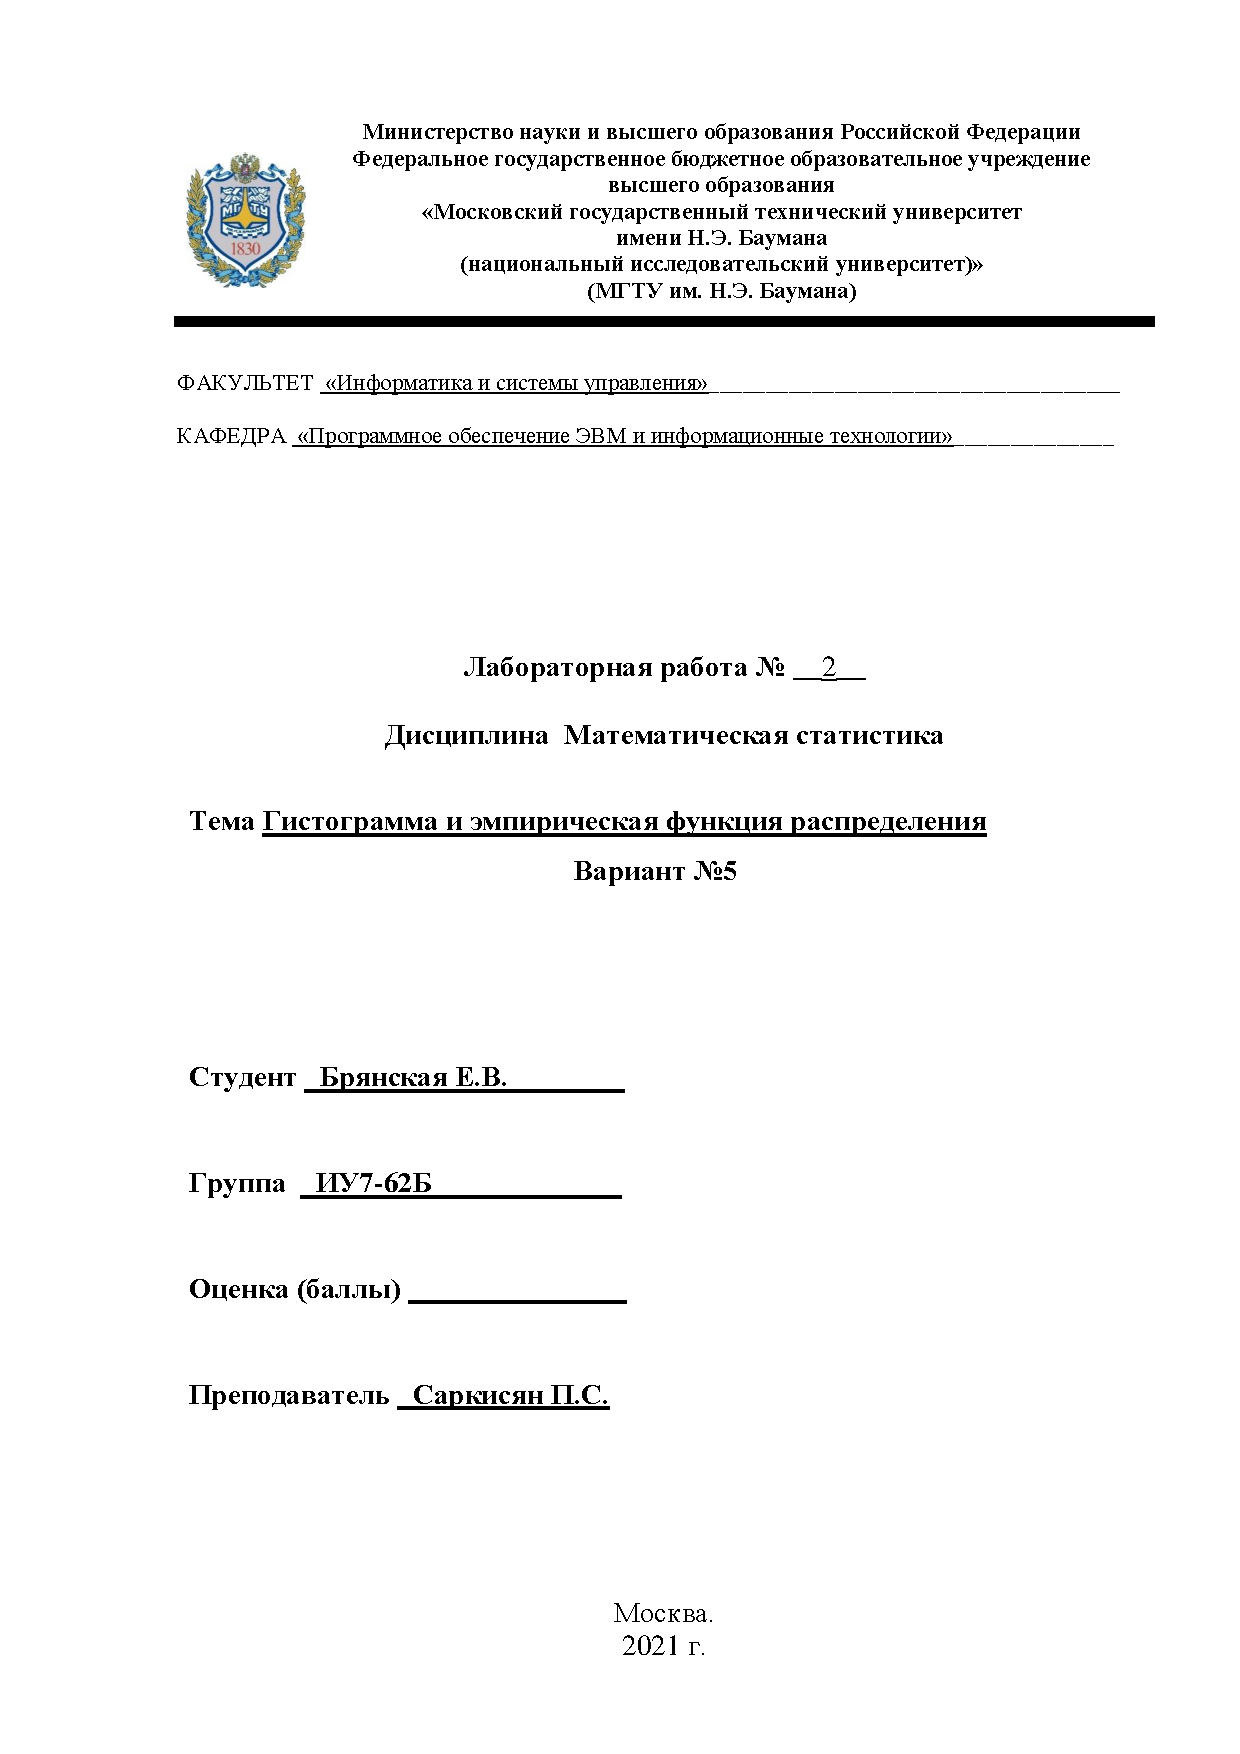
\includepdf[pages=1]{title.pdf}
	
	\tableofcontents
	\newpage
	
	\chapter*{Введение}
	\addcontentsline{toc}{chapter}{Введение}
	\textbf{Цель работы:} построение гистограммы и эмпирической функции распределения.
\textbf{Содержание работы:}

\begin{enumerate}
\item Для выборки объёма n из генеральной совокупности M реализовать в виде программы на ЭВМ
\begin{enumerate}
\item[а)] вычисление максимального значения $M_{max}$ и минимального значения $M_{min}$;
\item[б)] размаха R выборки;
\item[в)] вычисление оценок $\hat{\mu}$ и $S^2$ математического ожидания MX и дисперсии DX;
\item[г)] группировку значений выборки в m = [$log_2n$ ] + 2 интервала;
\item[д)] построение на одной координатной плоскости гистограммы и графика функции плотности распределения вероятностей нормальной случайной величины с математическим ожиданием $\hat{\mu}$ и дисперсией $S^2$;
\item[е)] построение на другой координатной плоскости графика эмпирической
функции распределения и функции распределения нормальной случайной величины с математическим ожиданием $\hat{\mu}$ и дисперсией $S^2$.
\end{enumerate}
\item Провести вычисления и построить графики для выборки из индивидуального варианта.

\end{enumerate}
	\newpage
	
	\chapter{Теоретическая часть}
	\section{Формулы для вычисления величин}
\subsection{Определение $\gamma$-доверительного интервала}
Доверительным интервалом уровня $\gamma$ для параметра $\theta$ называется интервал ($\underline\theta(\vec X)$, $\overline\theta(\vec X)$), образующий выборочными значениями статистики $\underline\theta$ и $\overline\theta$.\\
\begin{equation*}
	P\{\underline\theta(\vec X) <= x <= \overline\theta(\vec X) \} = \gamma
\end{equation*}

\section{Границы $\gamma$-доверительного интервала}

Пусть $\vec x = (x_1, ..., x_n)$ — случайная выборка объема $n$ из генеральной совокупности $X$, распределенной по нормальному закону с параметрами $\mu$ и $\sigma^{2}$.

\textbf{$\gamma$-доверительный интервал для математического ожидания}
\begin{equation*}
	P\{\overline{X} - \dfrac{S(\vec{X})}{\sqrt{n}} t^{St(n-1)}_{\frac{1+\gamma}{2}} <= \mu <= \overline{X} + \dfrac{S(\vec{X})}{\sqrt{n}} t^{St(n-1)}_{\frac{1+\gamma}{2}} \} = \gamma
\end{equation*}
Т.е.\\
\begin{equation*}
	\underline\mu(\vec X) = \overline{X} - \dfrac{S(\vec{X})}{\sqrt{n}} t^{St(n-1)}_{\frac{1+\gamma}{2}}
\end{equation*}

\begin{equation*}
	\overline\mu(\vec X)  = \overline{X} + \dfrac{S(\vec{X})}{\sqrt{n}} t^{St(n-1)}_{\frac{1+\gamma}{2}}
\end{equation*}

\subsection{Оценка для математического ожидания}

\textbf{$\gamma$-доверительный интервал для дисперсии}
\begin{equation*}
	P\{ \dfrac{S^2(\vec{X}) (n-1)}{t^{\chi^{2}(n-1)}_{\frac{1+\gamma}{2}}} <= \sigma^2 <= \dfrac{S^2(\vec{X}) (n-1)}{t^{\chi^{2}(n-1)}_{\frac{1+\gamma}{2}}}  \} = \gamma
\end{equation*}
Т.е.\\
\begin{equation*}
	\underline\sigma(\vec X) = \dfrac{S^2(\vec{X}) (n-1)}{t^{\chi^{2}(n-1)}_{\frac{1+\gamma}{2}}}
\end{equation*}

\begin{equation*}
	\overline\sigma(\vec X)  = \sigma^2 <= \dfrac{S^2(\vec{X}) (n-1)}{t^{\chi^{2}(n-1)}_{\frac{1+\gamma}{2}}}
\end{equation*}







	\newpage

	\chapter{Практическая часть}
	\section{Текст программы}

%\lstinputlisting[language=Matlab]{../lab1.m}


\section{Результат работы программы}


\section{Графики}
	\newpage
\end{document}
